%----------------------------------------------------------------------------------------
%	SECTION 1
%----------------------------------------------------------------------------------------

\section{The Base Axioms.}

\begin{definition}
    We call a maximally independent set of a matroid $M$ a \textbf{basis} of
    $M$.  We denote the collection of all bases of  $M$ to be  $\Bc$.
\end{definition}

\begin{lemma}\label{1.2.1}
    For any two bases $B_1$ and $B_2$ of a matroid, we have $|B_1|=|B_2|$.
\end{lemma}
\begin{proof}
    Suppose not, that $|B_1|<|B_2|$. Then, since $B_1,B_2 \in \Ic$, by
    augmentation, we can choose  $e \in \com{B_2}{B_1}$ such that $B_1 \cup e
    \in \Ic$. But $B_1$ is maximal, a contradiction! Terefore, $|B_1| \geq
    |B_2|$. Similarly, we get $|B_2| \geq |B_1|$.
\end{proof}

\begin{lemma}[The Base Axioms]\label{1.2.2}
    The collection $\Bc$ of bases of a matroid has the following properties:
    \begin{enumerate}
        \item[(B1)] $\Bc \neq \emptyset$.

        \item [(B2)] If $B_1,B_2 \in \Bc$, and $x \in \com{B_1}{B_2}$, then
            there exists $y \in \com{B_2}{B_1}$ such that $(\com{B_1}{x}) \cup y
            \in \Bc$.
    \end{enumerate}
\end{lemma}
\begin{proof}
    For (B1), if $\Bc=\emptyset$, then necesarrily,  $\Ic=\emptyset$, which
    cannot happen by (I1).

    Now, notice that both $\com{{B_1}}{x}$ and $B_2$ are independent, and that
    $|\com{B_1}{x}|<|B_2|$ by lemma \ref{1.2.1}. Therefore, by augmentation,
    take $y \in \com{B_2}{(\com{B_1}{x})}$, that is, $y \in \com{B_2}{B_1}$,
    such that $(\com{B_1}{x}) \cup y \in \Ic$. Then there is a basis $B' \in
    \Bc$ such that  $(\com{B_1}{x}) \cup y \subseteq B'$. Now, notice that
    $|(\com{B_1}{x}) \cup y|=|B_2|=|B'|$, thus $(\com{B_1}{x}) \cup y=B'$,
    makinng $(\com{B_1}{x}) \cup y \in \Bc$ a basis.
\end{proof}

With this lemma, we have proved that the independence axioms imply the base
axiom. We now show that the base axioms imply independence.

\begin{theorem}\label{1.2.3}
    Let $E$ be a finite set and  $\Bc \subseteq 2^E$ a collection of subsets of
    $E$ satisfying (B1) and (B2). let $\Ic=\{I \subseteq E : I \subseteq B,
    \text{ where } B \in \Bc\}$. Then $\Ic$ induces a matroid on  $E$.
\end{theorem}
\begin{proof}
    If  $\Bc \neq \emptyset$, then we have at least  $\emptyset \in \Ic$.
    Moreover, if $I_1 \in \Ic$, then $I_1 \subseteq B$, for some $B \in \Bc$.
    Then if  $I_2 \subseteq I_1$, $I_2 \subseteq B$ so that $I_2 \in \Ic$.

    Now suppose that $B_1,B_2 \in \Bc$ with $|B_1|>|B_2|$, such that
    $|\com{B_1}{B_2}|$ is minimal. Notice that $\com{B_1}{B_2} \neq \emptyset$,
    so choose $x \in \com{B_1}{B_2}$. Then by (B2), there exists a $y \in
    \com{B_2}{B_1}$ such that $(\com{B_1}{x}) \cup y \in \Bc$. Notice then that
    $|(\com{B_1}{x}) \cup y|=|B_1|>|B_2|$, so $|(\com{(\com{B_1}{x}) \cup
    y}{B_2})|<|\com{B_1}{B_2}|$ which contradicts minimality. So we have
    $|B_1|=|B_2|$.

    Now suppose that the augmentation axiom, (I3), fails. Then for $I_1,I_2 \in
    \Ic$ with $|I_1|<|I_2|$, there is an $e \in \com{I_2}{I_1}$ such that $I_1
    \cup e \notin \Ic$. Now, by definition, there exists $B_1,B_2 \in \Bc$ with
    $I_1 \subseteq B_1$ and $I_2 \subseteq B_2$. Choose, then, $B_2$ such that
    $|\com{B_2}{(B_1 \cup I_2)}|$ is minimal. Then
    $\com{I_2}{B_1}=\com{I_2}{I_1}$. Now, supposing that $\com{B_2}{(B_1 \cup
    I_2)} \neq \emptyset$, choose $x \in \com{B_2}{(B_1 \cup I_2)}$. Then by
    (B2), there exists a $y \in \com{B_1}{B_2}$ such that $(\com{B_2}{x}) \cup y
    \in \Bc$; but then $\com{((\com{B_2}{x}) \cup y)}{(B_1 \cup
    I_2)}<|\com{B_2}{(B_1 \cup I_2)}|$, which contradicts minimality. So
    $\com{B_2}{(B_1 \cup I_2)}=\emptyset$, and so
    $\com{B_2}{B_1}=\com{I_2}{B_1}$; that is:
    \begin{equation*}
        \com{B_2}{B_1}=\com{I_2}{I_1}
    \end{equation*}

    Now suppose that $\com{B_1}{(B_2 \cup I_1)} \neq \emptyset$. Then cor $x \in
    \com{B_1}{B_2 \cup I_1}$, there exists $y \in \com{B_2}{B_1}$ such that
    $(\com{B_1}{x}) \cup y \in \Bc$. Now, we have $I_1 \cup y \subseteq
    (\com{B_1}{x}) \cup y$, putting $I_1 \cup e \in \Ic$. Since $y \in
    \com{B_2}{B_1}$, we have $y \in \com{I_2}{I_1}$, which contradicts the
    hypothesis. So $\com{B_1}{(B_2 \cup I_1)}=\emptyset$. Thus,
    $\com{B_1}{B_2}=\com{I_1}{B_2}$. It follows then that $\com{B_1}{B_2}
    \subseteq \com{I_2}{I_1}$. Now, $|B_1|=|B_2|$, so
    $|\com{B_1}{B_2}|=|\com{B_2}{B_1}|$, thus
    $|\com{I_1}{I_2}|=|\com{I_2}{I_1}|$, so that $|I_1| \geq |I_2|$. but
    $|I_1|<|I_2|$, a contradiction. Therefore, (I3) must be satisfied, making
    $(E,\Ic)$ into a matroid.
\end{proof}
\begin{corollary}
    The matroid on $E$ induced by  $\Ic$ has  $\Bc$ as its collection of bases.
\end{corollary}

We now come to our next equivalent definition of a matroid.

\begin{definition}
    A \textbf{matroid} on a finite set $E$ is a pair $(E,\Bc)$, where $\Bc
    \subseteq 2^E$, such that:
    \begin{enumerate}
        \item[(B1)] $\Bc \neq \emptyset$.

        \item [(B2)] If $B_1,B_2 \in \Bc$, and $x \in \com{B_1}{B_2}$, then
            there exists $y \in \com{B_2}{B_1}$ such that $(\com{B_1}{x}) \cup y
            \in \Bc$.
    \end{enumerate}
    We call $\Bc$ the collection of \textbf{bases} of the matroid.
\end{definition}
\begin{corollary}
    For any $B \in \Bc$ and $e \in \com{E}{B}$, $B \cup e$ contains a unique
    circuit  $C(e,B)$ which contains $e$.
\end{corollary}
\begin{proof}
    This follows immediately from the analogous corollary to theorem
    \ref{1.1.3}.
\end{proof}

\begin{definition}
    Let $M$ be a matroid with ground set $E$ and collection of bases $\Bc$. For
    $e \in \com{E}{B}$, we define the \textbf{fundamental circuit} of $e$ with
    respect to  $B$ to be the circuit $C(e,B)$ with the property that $e \in
    C(e,B) \subseteq B$.
\end{definition}

\begin{lemma}[Fundamental Circuit Theorem.]\label{1.2.4}
    Every circuit of a matroid is the fundamental circuit of some element with
    respect to some basis.
\end{lemma}
\begin{proof}
    Let $C$ be a circuit of some matroid $M$, and choose $e \in C$. Then choose
    some basis $B$ of  $M$ in which  $e \in \com{E}{B}$ ($E$ the ground set of
    $M$). Then by the corollary to theorem \ref{1.2.3}, we have that there is a
    circuit $C(e,B)$ such that $e \in C(e,B) \subseteq B \cup e$. We then have
    that $e \in C \subseteq B \cup e$, and that  $e \in C \cap C(e,B)$. Then by
    weak circuit elimination, there is a circuit $C' \subseteq \com{(C \cup
    C(e,B))}{e}$. Then $C' \subseteq \com{C}{e}$ and $C' \subseteq
    \com{C(e,B)}{e}$. That is $C' \cup e \subseteq C$ and  $C' \cup e \subseteq
    C(e,B)$. Thus, either $C \subseteq C(e,B)$ or $C(e,B) \subseteq C$; in
    either case we get $C=C(e,B)$.
\end{proof}

\begin{example}\label{1.9}
    \begin{enumerate}
        \item[(1)] let $m,n \in \Z^+$ with  $m \leq n$. Let  $E$ be an
            $n$-element set, and  $\Bc$ the collection of all  $m$-element
            subsets of  $E$. Then  $\Bc$ is the collection of bases for a
            matroid on  $E$.

            Notice that since  $|E|=n$, and  $m \leq n$, then there exists at
            least on  $m$-element subset of $E$, so that $\Bc \neq \emptyset$.
            Now, let $B_1,B_2 \in \Bc$ be distinct with $|B_1|=|B_2|=m$. Then
            for $x \in \com{B_1}{B_2}$, notice that $|\com{B_1}{x}|=m-1$. Thus,
            choose $y \in \com{B_2}{B_1}$ (which exists), then $|(\com{B_1}{x})
            \cup y|=m$, making $\com{B_1}{x} \cup y \in \Bc$. Then $(E,\Bc)$
            forms a matroid which we call the \textbf{uniform matroid} of rank
            $m$ on an $n$-element set. We denote the uniform matroid by
            $U_{m,n}$.

        \item[(2)] In the uniform matroid, $U_{m,n}$, we have the collection of
            independent sets is given by:
            \begin{equation*}
                \Ic=\{X \subset E : |X| \leq m\}
            \end{equation*}
            and the collection of circuits is given by $\Cc=\emptyset$ if
            $m=n$, or
            \begin{equation*}
                \Cc=\{X \subseteq E : |X|=m+1\}.
            \end{equation*}
            if $m<n$.

        \item[(3)] If $m=0$, then the only independent sets of  $U_{0,n}$ are
            emptysets, i.e. $\Ic=\Bc=\{\emptyset\}$. This makes all $n$-elements
            of the ground set loops. Likewise, if  $m=1$, then the only
            independent sets of  $U_{1,n}$ are singletons, hence $U_{1,m}$
            consists of $n$ parallel elements. If  $m \geq 2$, then $U_{m,n}$ is
            simple.

        \item[(4)] $U_{n,n}$ has no circuits, since by above, $\Cc=\emptyset$,
            and $U_{0,0}=\emptyset$ the empty matroid.
    \end{enumerate}
\end{example}

\begin{definition}
    We call a matroid $M$  \textbf{free} if its collection of circuits is empty.
\end{definition}

\begin{example}\label{1.10}
    \begin{enumerate}
        \item[(1)] Let $E$ be a nonempty set and  $(E_1, \dots, E_r)$ be a
            partition $\pi$ of  $E$ into nonempty subsets. Let  $\Bc$ be the
            collection of all suubsets of  $E$ containing exactly one element of
             $E_i$ for each  $1 \leq i \leq r$. Then $\Bc$ is the collection of
             bases of a matroid on $E$ called the \textbf{partition matroid},
             $M_\pi$.

         \item [(2)] $M_\pi$ has as its collection of independent sets, bases,
             and circuits given by:
             \begin{align*}
                 \Ic &= \{X \subseteq E : |X \cap E_i| \leq 1, \text{ for all }
                 1 \leq i \leq r\} \\
                 \Bc &= \{X \subseteq E : |X \cap E_i|=1, \text{ for all }
                 1 \leq i \leq r\} \\
                 \Cc &= \{\{a,b\} \subseteq E : \{a,b\} \subseteq E_i, \text{
                 for all } 1 \leq i \leq r\} \\
             \end{align*}

         \item[(3)] If $|E_i|=1$ for all  $i$, then  $M_\pi \simeq U_{r,r}$. In
             general. we also have that $M_\pi$ is graphic, as it is isomorphic
             to the cycle matroid of a vertex-disjoint union of graphs $G_1,
             \dots, G_r$ where $G_i$ consists of  $2$ vertices joined by $|E_i|$
             distinct edges.
    \end{enumerate}
\end{example}

\begin{example}\label{1.11}
    \begin{enumerate}
        \item[(1)] Let $G$ be a graph. Then a subset $X \subseteq E$ of edges
            of $G$ is independent if, and only if they from a forest of the
            graph $G$. Then $X$ is a basis if  $X$ is a forest such that for
            $e \in \com{E}{X}$, $X \cup e$ contains a cycle. That is, $X$ forms
            a spanning tree in all connected components of  $G$. If  $G$ is
            connected, then $X$ is a spanning tree. Likewise, it can be shown
            that spanning trees are bases, so that we have that  $X$ is the
            basis of matroid on a graph $G$ if, and onlt if it forms spanning
            trees across all connected components of $G$.

        \item [(2)] Let $A$ be an $m \times n$ matrix over a field $F$. Then the
            columns of  $A$ span a subspace  $W$ of dimension  $r$. We also see
            that independent sets of columns of $A$ are linearly independent.
            Thus, if we have a subset of columns of $A$, linearly independent,
            also spanning the subspace $W$, they form a basis of  $W$. That is,
            a set $B$ of columns of  $A$ forms a basis for  $W$ if, and only if
             $B$ is linearly independent, and $|B|=r$; so that $B$ is a set of
             basis vectors for the subspace $W$.

         \item[(3)] If $A=\begin{pmatrix}
                        1 & 0 & 1 & 1 \\
                        0 & 1 & 1 & 2 \\
                      \end{pmatrix}$
                is a $2 \times 4$ matrix over $\F_3$, then $\dim{W}=2$, and so
                the bases are all $2$ element subsets of linearly independnet
                columns. Thus  $M(A) \simeq U_{2,4}$.
    \end{enumerate}
\end{example}

\begin{theorem}\label{1.2.5}
    Let $M$ be a graphic matroid. Then $M$ is isomorphic to the cycle matroid of
    some connected graph $G$.
\end{theorem}
\begin{proof}
    Let $M$ be a matroid, and dentoe the cycle matroid of any graph $G$ by
    $M(G)$. Then $M \simeq M(H)$ for some graph $H$. If  $H$ is connected, we
    are done.

    Now suppose that  $H$ is not connected. Consider then the connected
    components  $H_1, \dots, H_n$ of $H$. Choose a vertex  $v_i \in H_i$ and
    form the graph  $G$ with vertices  $v_1, \dots, v_n$ all labeled as one
    vertex. Then the edge set $E(H)=E(G)$ the edge set of $G$; moreover, $X
    \subseteq E(G)$ is a cycle if, and only if it is a cycle in $E(H)$. Thus we
    have $M \simeq M(H)$.
\end{proof}

To finish the section, we make the following observation. The independence,
base, and circuit axioms constitute the three main equivalent ways of definining
a matroid. We can denote these definitions as $(\Ic)$, $(\Bc)$, and $(\Cc)$.
Now, by theorems \ref{1.1.3} and  \ref{1.2.3}, we have that $(\Ic)$ is
equivalent to  $(\Bc)$ and $(\Cc)$. Moreover, notice that $(\Bc)$ implies
$(\Ic)$, and $(\Ic)$ implies $(\Cc)$. Thus, by transitivity of implication,
$(\Bc)$ implies $(\Cc)$. Conversely, we have that $(\Cc)$ implies $(\Ic)$, which
implies $(\Bc)$. So by transitivity again, we get that $(\Cc)$ implies $(\Bc)$.
Therefore $(\Bc)$ and $(\Cc)$ are equivalent definitions of a matroid. Collecting
our definitions into a digraph, whose edge set is given by implication,
we get the following figure:
\begin{remark}
    That is, two vertices $a,b$ in the digraph form an edge  $(a,b)$ if $a$
    implies  $b$.
\end{remark}

\begin{figure}[h]
    \centering
    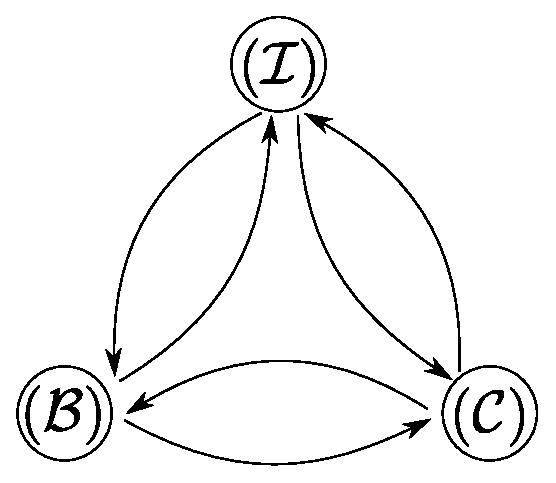
\includegraphics[scale=0.5]{Figures/Chapter1/equiv_def_1.eps}
    \caption{The implication digraph of $(\Ic)$, $(\Bc)$, and $(\Cc)$.}
    \label{fig_1.3}
\end{figure}
